%%%%%%%%%%%%%%%%%%%%%%%%%%%%%%%%%%%%%%%%%%%%%%%%%%%%%%%%%%%%%%%%%%%%
\section{Transport and Receiving at the DUNE Integration Facility}
\label{sec:fdsp-apa-transport}

Completed \dwords{apa} are shipped from the \dword{apa} production sites to an \dword{itf} where they will be integrated with the TPC \dword{fe} electronics and \dwords{pd}.  The \dword{itf} location is not yet confirmed, but facilities near the \surf site are being considered.   Activities at the \dword{itf}  include extensive \dword{qc} testing to ensure the fully integrated \dwords{apa} function properly.  Once checked, the \dword{apa}s are repackaged for final transport to \surf.  For details on installation activities at \surf, see the Technical Coordination chapter in this TDR.  Here we limit the discussion to delivery of \dword{apa}s to the \dword{itf} and quality checks once there to ensure each \dword{apa} has arrived without damage. 

%Each \dword{apa}, still in its transport crate, is hung from the Ross Shaft cage using a sling and transported underground where it is stored in a holding area.  Pairs of \dwords{apa} must be linked in their vertical configuration and cables run from both the lower and upper \dwords{apa} in an area just outside the cryostat.  Once that is completed, the pairs enter through the \dword{tco} onto the \dword{dss} and are moved into their final position.  Final checkout tests are performed once the \dwords{apa} are in place.

%We expect to integrate the assemblies with the \dwords{pd} at the Integration Facility. %However, as an alternative, they could be installed at the \dword{apa} production sites (the specifics of the plan must be developed with the \dword{pds} consortium and depend on the final \dword{pds} design). 
%An alternative plan entails installing the \dword{pds} at the \dword{apa} production sites. The TPC \dword{fe} electronics are installed  at the \dword{itf}, and the exact installation sequence will be developed with the electronics consortium.

%A conceptual layout of the space required at the Integration Facility is being developed. An overhead crane is needed to lift \dwords{apa} out of their shipping crates and maneuver them through the facility.  Most of the handling areas must be embedded in a class \num{100000} clean tent. Finally, a cold box will be available to test the \dword{qc} electronics once they are installed on the \dword{apa} (see Section~\ref{sec:fdsp-apa-install-qc_if}).  

%\begin{dunefigure}[Schematics of the layout of the \dword{itf} testing area]{fig:testlayout}{A schematic of the layout for the testing area at the \dword{itf}. Most of this area has to be embedded in a clean environment (i.e. tent).}
%%\includegraphics[width=0.4\textwidth]{test_layout.png} 
%\end{dunefigure}


%%%%%%%%%%%%%%%%%%%%%%%%%%%%%%%%%%%%%%%%%%%%%%%%%%%%%%%%%%%%%%%%%%%%
\subsection{APA Handling}
\label{sec:fdsp-apa-transport-handling}

%\begin{dunefigure}[Draft of the \dword{apa} transport crates]{fig:crate}{A schematic design of the \dword{apa} transport crate (note that the material will not be wood).}
%%\includegraphics[width=0.5\textwidth]{tp3-5-1-fig1.jpg} 
%\end{dunefigure}

The handling of the \dwords{apa} throughout their lifetime must be carefully considered to ensure their safety.  Several lifting and handling fixtures will be employed for transferring and manipulating the \dword{apa}s during fabrication, integration and installation.  In the factories a fixture called the `edge lift kit' will be used to transfer the APA to and from the process cart and the winder, and to the transport containers.  See Figure~\ref{fig:apa-edge-lift}.  The edge lift kit will also be used in the integration facility to transfer the APA from the transport frame to a process cart there.  

\begin{dunefigure}[\dword{apa} edge lifting fixture]{fig:apa-edge-lift}
{Custom listing fixture used to safely handle the \dword{apa} during the various construction steps at the factories.}  
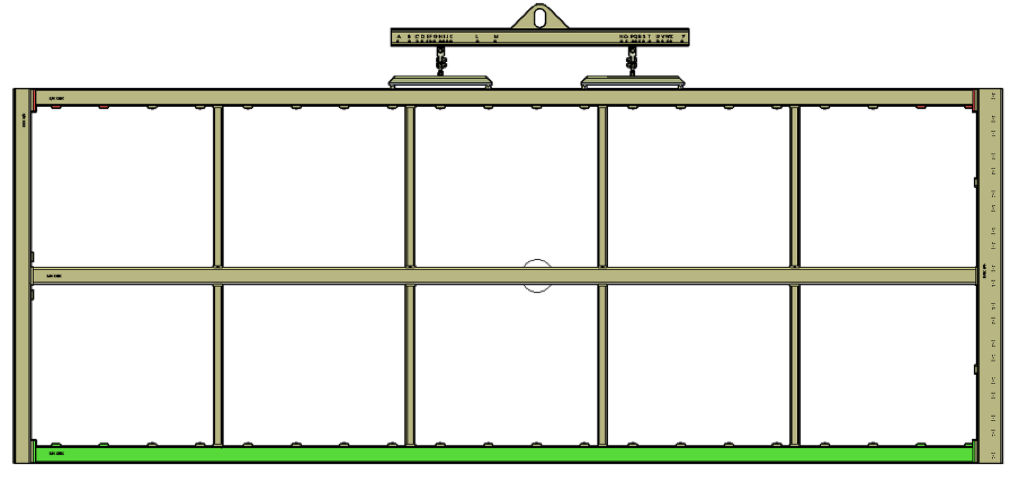
\includegraphics[width=0.8\textwidth]{sp-apa-edge-lift-kit.png} 
\end{dunefigure}

Discussion of the handling of \dword{apa}s from the \dword{itf} to \surf and into the cryostat can be found in the Technical Coordination chapter. 

%\fixme{PSL: need a little text on handling and any lifting fixtures or procedures to be mentioned.}

%at the \dword{itf} and underground is done with overhead cranes. Once the \dwords{apa} are repackaged in the crates, they are loaded onto a truck, driven to the mine, transported to the cage, secured to the sling under the cage (see figure \ref{fig:cagetransport}), lowered, and moved to the underground storage area.

%\begin{dunefigure}[\dword{apa} suspended beneath the mine shaft cage]{fig:cagetransport}{The \dword{apa} crate (in blue) is brought underground with a sling under the elevator cage (the green box at the top of the figure). The insertion into the crate at the surface is done from the back of the cage, but the extraction underground must be done from the front of the cage. The \dword{apa} crate must, therefore, be able to be rotated  by 180$^\circ$ in the sling.}
%\setlength{\fboxsep}{0pt}
%\setlength{\fboxrule}{0.5pt}
%\fbox{\includegraphics[width=0.4\textwidth, trim=0mm 20mm 0mm 20mm,clip]{apa-cage.jpg}}
%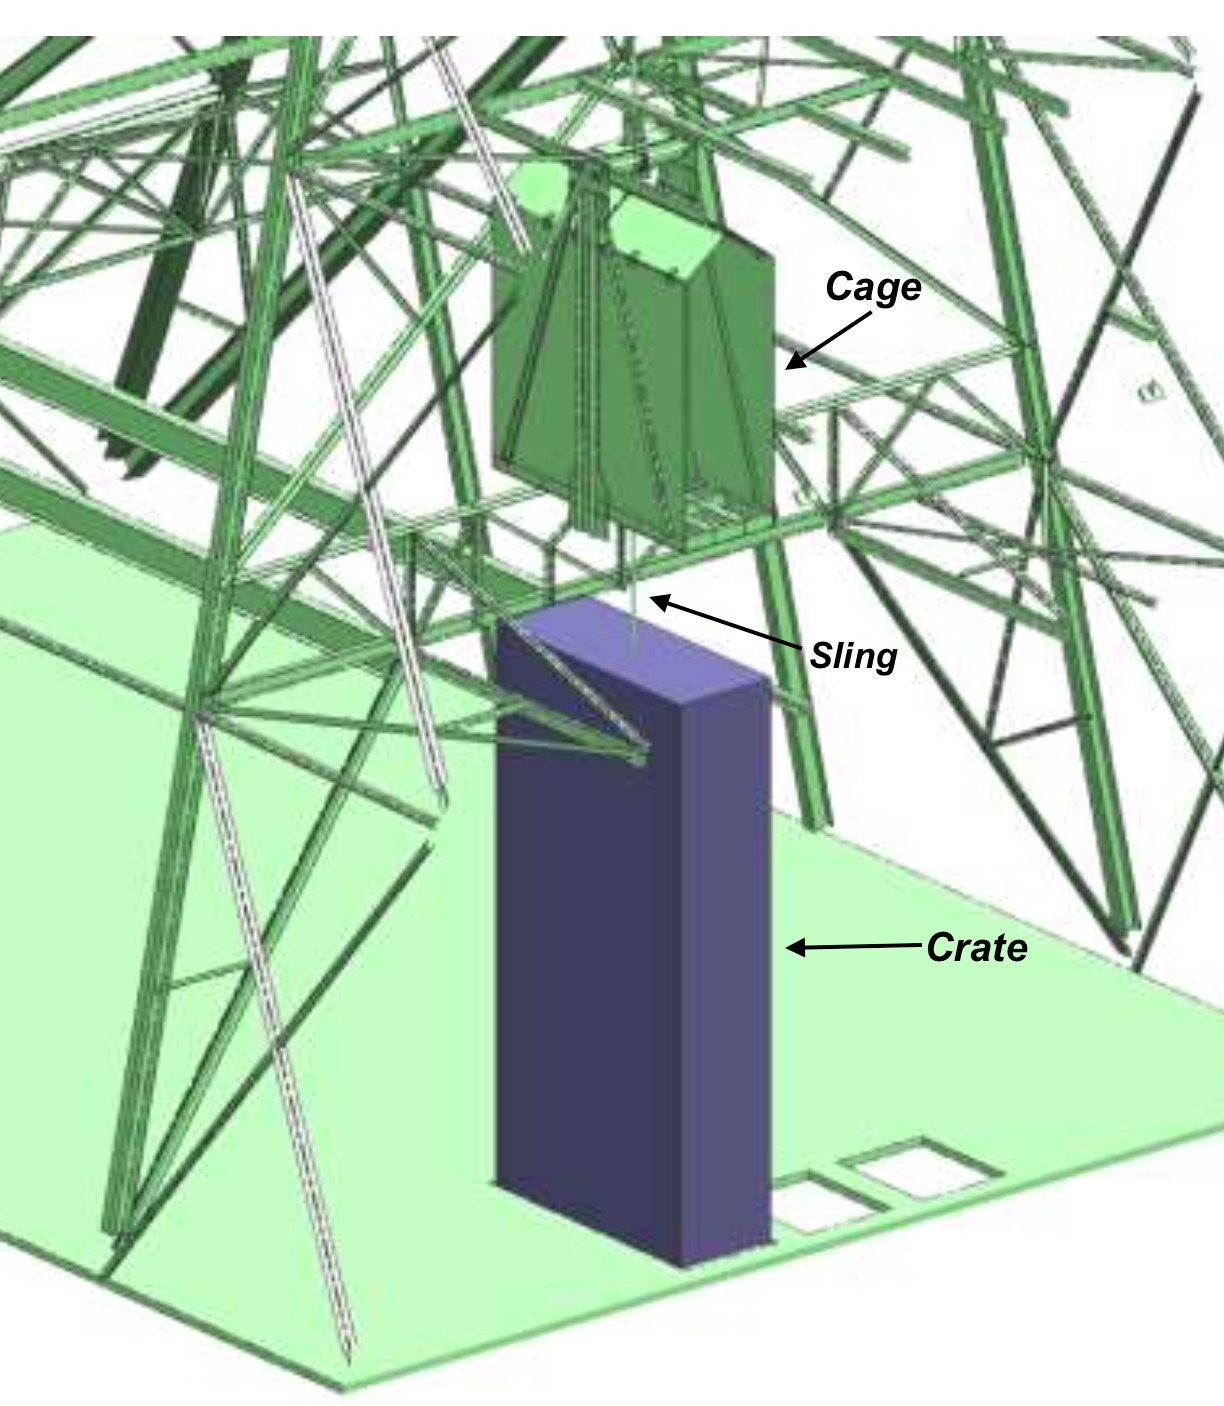
\includegraphics[width=0.4\textwidth, trim=0mm 20mm 0mm 20mm,clip]{sp-apa-cage.jpg}
%\end{dunefigure}



\subsection{APA Transport Frame and Shipping Strategy}
\label{sec:fdsp-apa-transport-container}

%Custom designed crates will be used to transport the completed \dword{apa}s between the production sites and the \dword{itf}. 

%***This is an active area of study and design.***

The purpose of the \dword{apa} transport frame is to provide a safe and strong transport environment to send \dword{apa}s  from production sites to the \dword{itf}. The main requirements are to provide an enclosure for a pair of \dword{apa}s, allow lifting and rotating to many different positions, and be compact enough to go down the shaft at \surf. 

Figure~\ref{fig:apa-transport-frame} shows the current concept for a transport frame, which comprises of a central support and a left and right hand bolted-on cage.  The \dword{apa}s are connected to the central support by means of two sets of vertical spring struts. These are sprung to allow for anti-vibration and reduce any shock loads to the \dword{apa}s when being transported. 

\begin{dunefigure}[\dword{apa} transport frame]{fig:apa-transport-frame}
{Transport frame concept for transporting two \dword{apa}s between a production site and the \dword{itf} and between the \dword{itf} and \surf for installation.}  
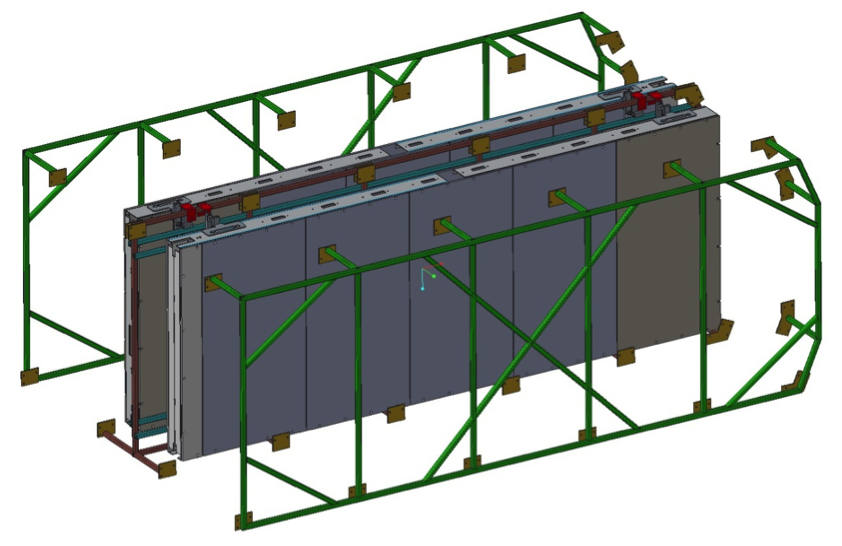
\includegraphics[width=0.8\textwidth]{sp-apa-transport-frame.png} 
\end{dunefigure}

Work is ongoing to finalize the transport crate design and plan the details of the transport procedures.

\begin{comment}
The spring system is shown in Fig.~\ref{fig:apa-transport-springs}. It comprises of two vertical struts with 3 springs per pair. The `wire rope' springs are Cavoflex and are manufactured by Vibrostop. Vibrostop will perform the relevant calculations based on input data such as methods of travel (by road or by sea) and lifting operations when loading onto a trailer or being manipulated down the shaft at \surf.

\begin{dunefigure}[\dword{apa} transport frame spring system]{fig:apa-transport-springs}
{Transport frame designed to transport two \dword{apa}s between production sites and the \dword{itf} and \surf.}  
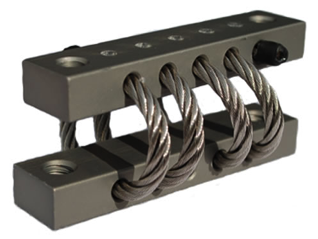
\includegraphics[height=0.19\textheight]{sp-apa-transport-spring.png} \qquad
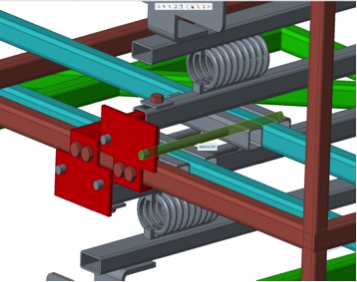
\includegraphics[height=0.2\textheight]{sp-apa-transport-detail.png} 
\end{dunefigure}
\end{comment}

%\fixme{Peter, Alberto: are these reused and sent back to production sites? No, too costly to ship back to UK.  In US, less clear, may reuse them. An APA lives in this frame until it reaches underground.  it may be possible to reuse some of them (at least in the US).  What we show here is the current concept, but will evolve along with final plans for the ITF.}
%\fixme{Peter: providing text and engineering drawings showing the crate design.}

%The crate design is not yet finished, but we have two possible approaches. The first is to use less expensive, disposable crates for transport to the \dword{itf} and fewer, more expensive crates for transport underground. The more expensive crates are reused between the \dword{itf} and underground. The second option is a single crate used for all transport stages. Transport underground requires a design that allows a 180$^{\circ}$ rotation of the crate. 



\begin{comment}
%%%%%%%%%%%%%%%%%%%%%%%%%%%%%%%%%%%%%%%%%%%%%%%%%%%%%%%%%%%%%%%%%%%%
\subsection{APA-to-CPA Assembly and Installation in the Cryostat}
\label{sec:fdsp-apa-install-cryostat}

Once underground, there will be a small storage area for stockpiling \dwords{apa} (see Figure~\ref{fig:handling}). When ready for installation, each \dword{apa} is extracted from its crate, inspected and rotated to be lowered into the area just outside of the \dword{tco} in the cryostat. Two \dwords{apa} are lowered in front of the \dword{tco} where they are linked and cabled. The details of the cabling are still being finalized, but the main option is currently to pass all the cables inside the \dword{apa} frame tubes (see Section~\ref{sec:fdsp-apa-intfc-apa}).

%\begin{dunefigure}[\dword{apa} cabling]{fig:\dword{apa}cables}{Proposed cabling solution for the \dwords{apa}. }
%\begin{tabular}{cc}
%%\includegraphics[width=0.5\textwidth]{\dword{apa}_cables_2.png} 
%%\includegraphics[width=0.4\textwidth]{\dword{apa}_cables.jpeg} 
%\end{tabular}
%\end{dunefigure}

%\begin{dunefigure}[\dwords{apa} in the \dword{tco}]{fig:\dword{apa}_\dword{tco}}{Left: Top and bottom \dwords{apa} placed in the \dword{tco} for cabling and linking. Center: Linking bracket current design. Right: Current \dword{apa} linking solution.}
%\begin{tabular}{cc}
%%\includegraphics[width=0.3\textwidth]{\dword{apa}_link.png} 
%%\includegraphics[width=0.4\textwidth]{\dword{apa}_link_2.png} 
%\end{tabular}
%\end{dunefigure}

Finally, when the two \dwords{apa} are fully cabled, they are placed onto the DSS inside the cryostat (see bottom right of Figure~\ref{fig:handling}) and moved to their location in the cryostat where final integration tests are performed.  For more information on the detector support structure and installation into the cryostat, see %the Technical Coordination 
Chapter~\ref{ch:fdsp-coord}. 

\begin{dunefigure}[Underground handling of the \dwords{apa}]{fig:handling}{(Top row) Handling of an \dword{apa} in the underground storage area where the \dwords{apa} are extracted from the crates, inspected, and readied for installation in the cryostat. (Bottom row) A pair of \dwords{apa} are brought into the space just outside the \dword{tco} to be linked and cabled, then connected to the \dword{dss} and moved into their final position inside the cryostat.}
\setlength{\fboxsep}{0pt}
\setlength{\fboxrule}{0.5pt}
\centering
\fbox{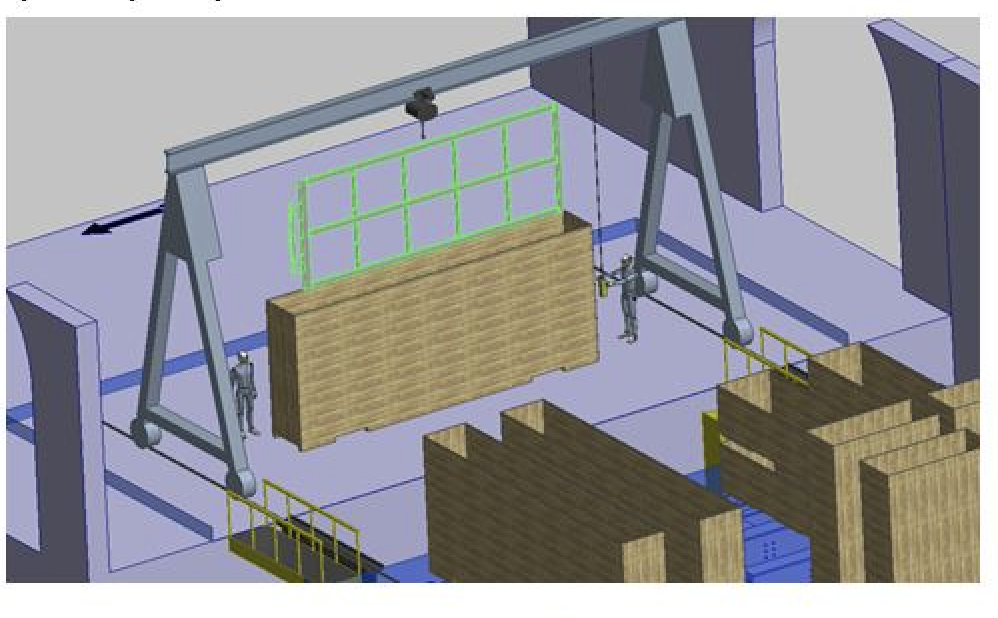
\includegraphics[height=0.195\textheight,trim=8mm 8mm 20mm 4mm,clip]{sp-apa-install-1.png}} 
\fbox{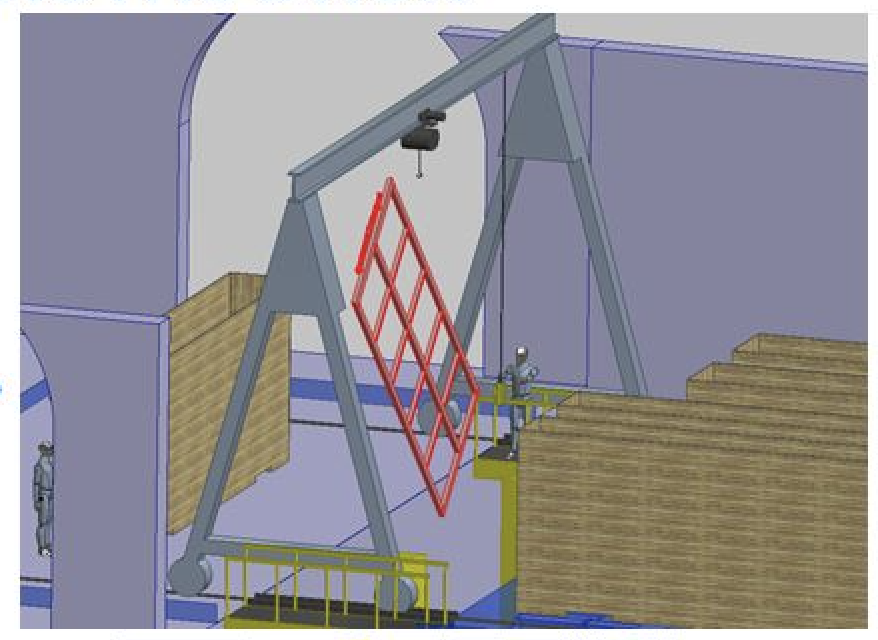
\includegraphics[height=0.195\textheight,trim=8mm 4mm 20mm 4mm,clip]{sp-apa-install-2.png}} 
\fbox{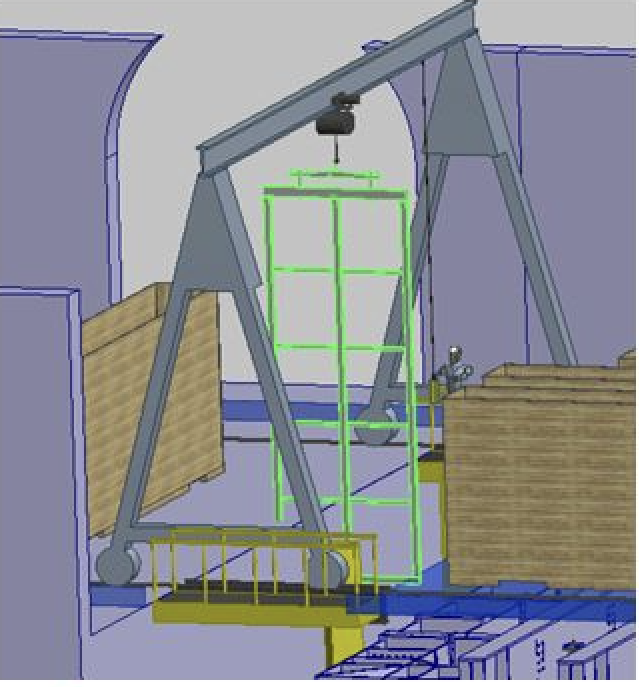
\includegraphics[height=0.195\textheight,trim=4mm 4mm 4mm 4mm,clip]{sp-apa-install-3.png}} 
\\ \vspace*{1.5mm}
\hspace*{-.25mm}
\fbox{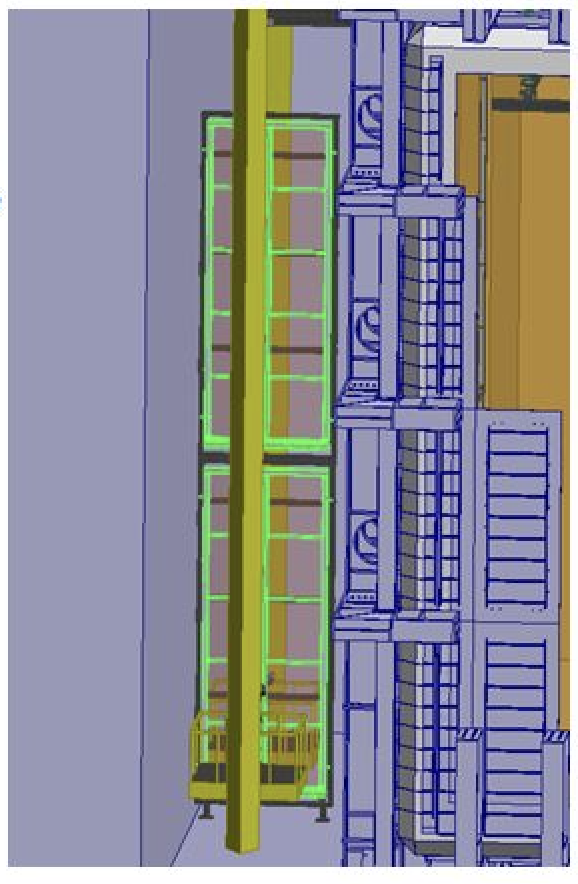
\includegraphics[height=0.37\textheight,trim=4mm 4mm 4mm 4mm,clip]{sp-apa-install-4.png}}
\hspace*{1.mm}
\fbox{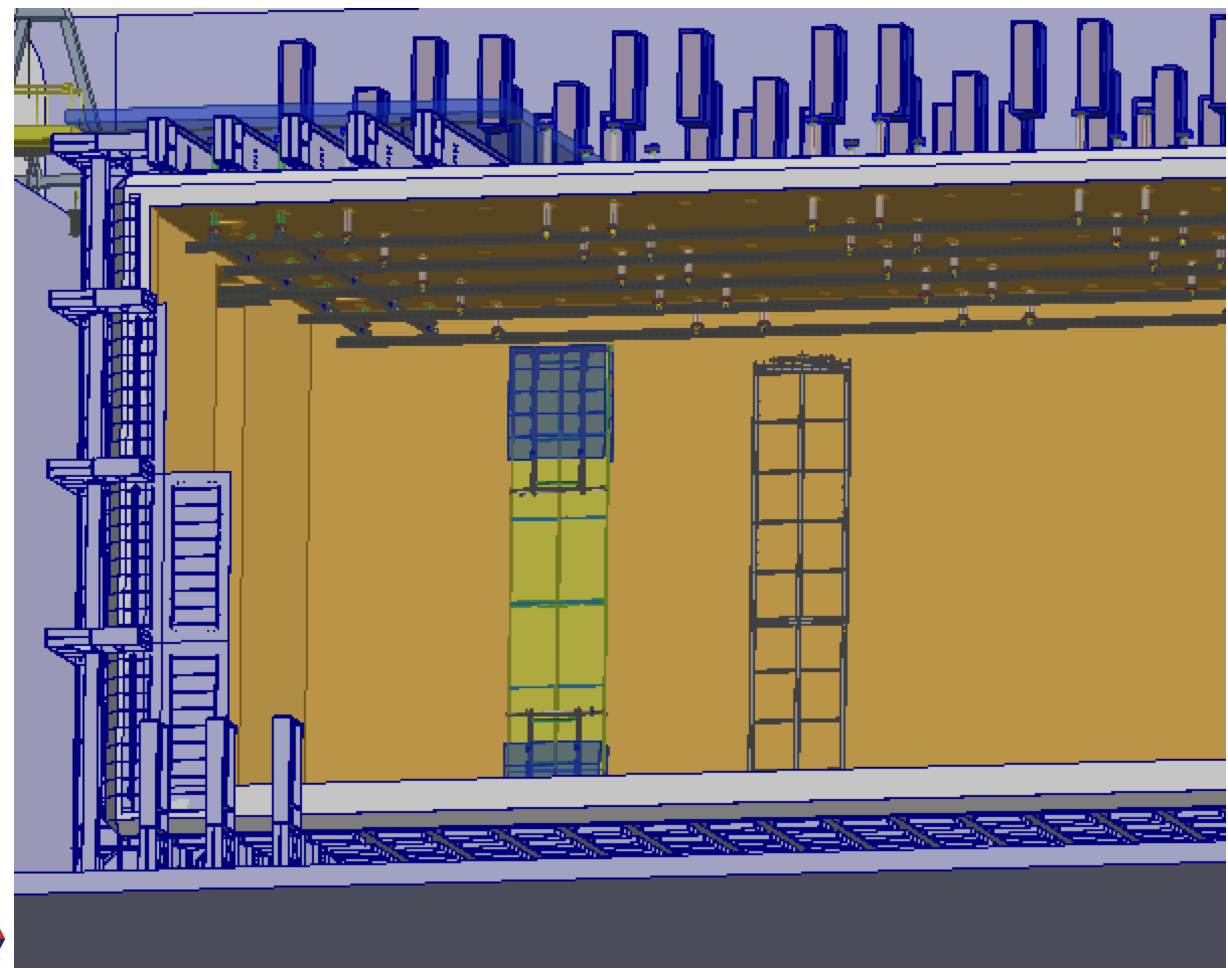
\includegraphics[height=0.37\textheight,trim=4mm 4mm 4mm 4mm,clip]{sp-apa-install-5.png}}
\end{dunefigure}
%\begin{dunefigure}[\dwords{apa} in the cryostat]{fig:\dword{apa}_cryostat}{Top/bottom \dword{apa} pairs are moved inside the cryostat to their final location.}
%%\includegraphics[width=0.5\textwidth]{\dword{apa}_cryostat.png} 
%\end{dunefigure}
\end{comment}

%%%%%%%%%%%%%%%%%%%%%%%%%%%%%%%%%%%%%%%%%%%%%%%%%%%%%%%%%%%%%%%%%%%%
\subsection{Quality Control at the DUNE Integration Facility}
\label{sec:fdsp-apa-transport-qc}

%\fixme{Roxanne, Jonathan: review and update text}

\begin{comment}
The \dword{qc} of integration and installation has two main testing campaigns: one at the Integration Facility (\dword{itf}) \fixme{from Nora: This has been defined once already and need not be defined again.} and one once the \dwords{apa} are installed into the cryostat. The installation and integration team in the \dword{apa} consortium are still developing some details. 

To keep track of all components for all \dwords{apa} at the different stages of  integration and installation requires a dedicated database for \dword{qc}. For efficient integration, a simple and practical way of tagging critical parts in the \dword{apa} is also being developed.

The \dword{qa} for integration and installation relies heavily on the \dword{pdsp} experience, and at this point, no dedicated \dword{qa} protocol is developed. The full development of the protocol is being handled by the installation and integration team in the \dword{apa} consortium. 

%%%%%%%%%%%%%%%%%%%%%
\subsubsection{Quality Control at the Integration Facility}
\label{sec:fdsp-apa-install-qc_if}
\end{comment}

All active detector components are shipped to the \dword{itf} for integration and testing; there we will have more time available %. It is at that location that we will have the most time 
to perform tests. This step is critical for ensuring high performance of the integrated \dwords{apa}. The exact time scale of \dword{apa} testing must be finalized using information from the production sites and the installation schedule. 


%Table \ref{tab:qclist} shows a summary of the quality control tests that will be performed at the \dword{itf}. The details of each is given below. %Figure \ref{fig:testlayout} shows an example of the layout of the testing area at the \dword{itf}.

\begin{comment}
\begin{dunetable}[QC List]{l|c|c}{tab:qclist}{List of tests performed for Quality Control upon reception at the integration facility}   
Test to perform   &  Number of wires/channels & Acceptable values, action\\ 
Visual inspection & All & > 99\% intact \\
Wire tension      & 10$\%$ sample & 5 $\pm$ \SI{1}{N}\\
Wire continuity   & All & $-$\\
Current leakage   & All & < X $\mu$A \\
Electronics connections & All & Perfect (> 99$\%$)\\
%Noise             & All &  $\pm$ XX (> 99$\%$)\\
Cold test         & All & All intact (> 99$\%$)\\
\textbf{Overall}  & \textbf{All} & \textbf{At least 99$\%$ fully operational}\\
\end{dunetable}
\end{comment}

After unpacking an \dword{apa} at the \dword{itf}, a thorough visual inspection will be performed. Tension measurements will be made for a sample of approximately $\sim$10\% of the wires (around \num{350} wires). The default technique is the laser method that was used for \dword{pdsp}.  The method works well, but it is time consuming, so alternatives that use voltage measurements are also being pursued to reduce the time spent on measuring. Improved methods could allow measurement of more wires (even the full \dword{apa}). 

Tension values are recorded to the database and compared with the original tension measurements performed at the production sites, as was done for \dword{pdsp} and shown in Fig.~\ref{fig:sp-apa-pd-tension} . Definite guidance for the acceptable tension values will be available to inform decisions on the quality of the \dword{apa}. Clear pass/fail criteria % I think slash ok in this construction; leaving it in (anne)
will be provided as well as clear procedures to deal with individual wires lying outside the acceptable values. %Exact relation between lower or higher tension and the acceptance of a channel still needs to be worked out. 
This guidance will be based on the \dword{pdsp} experience, where the tension of some wires changed during the production to installation process. In addition, a continuity test and a leakage current test is performed on all the wires, and the data recorded to the database. 

%Once the electronics are installed by the electronics consortium, dedicated testing of the \dword{apa} readout is performed. The integrated \dword{apa} is placed in the cold box so the performance of the electronics can be adequately tested. 
%Strict guidance is provided %will be available to for assessing the pass/fail criteria for each \dword{apa} during these tests. 
%The pass/fail criteria will provide strict guidelines for assessing each \dword{apa} during these tests. Here too, experience from \dword{pdsp} and development tests will establish the exact criteria. Close collaboration with the electronics consortium is necessary.

When all tests are successful and more than \num{99}\,\% of the channels are confirmed functional, the \dword{apa} can be prepared for integration with the other components and shipment to \surf{}.  The details of integration and installation can be found in the chapter on Technical Coordination.  A set of final checks, following installation in the cryostat, will definitely be performed to confirm the function of the \dword{apa}s in their final positions.

\begin{comment}
%%%%%%%%%%%%%%%%%%%%%%%%%%
\subsubsection{Quality Control Underground}
\label{sec:fdsp-apa-install-qc_underground}

We have three opportunities to test the \dwords{apa} underground: in the storage area, once secured in front of the \dword{tco}, or once positioned at their final location in the cryostat. The last is the most important, and we may save time by performing the final tests once the full \textit{APA-CPA-APA-CPA-APA} wall is installed (\dwords{cpa} are described in Chapter~\ref{ch:fdsp-hv}). This does risk, if serious problems are found, moving the \dwords{apa} out again, which may be harder and more time-consuming.

%\paragraph{Tests underground in the storage/unpacking area}
The \dwords{apa} are unpacked in the underground storage area (see Figure~\ref{fig:storage}). Space in this area is very limited, so only visual inspection is performed during unpacking. If clear defects are visible, the \dword{apa} is returned to the \dword{itf} for further investigation.

\begin{dunefigure}[Schematics of the underground storage area; full A-C-A-C-A wall in the cryostat]{fig:storage}{Left: A schematic of the layout for the underground storage and unpacking area. Right: A schematic of the layout of a full APA-CPA-APA-CPA-APA wall installed in the cryostat.}
\setlength{\fboxsep}{0pt}
\setlength{\fboxrule}{0.5pt}
\fbox{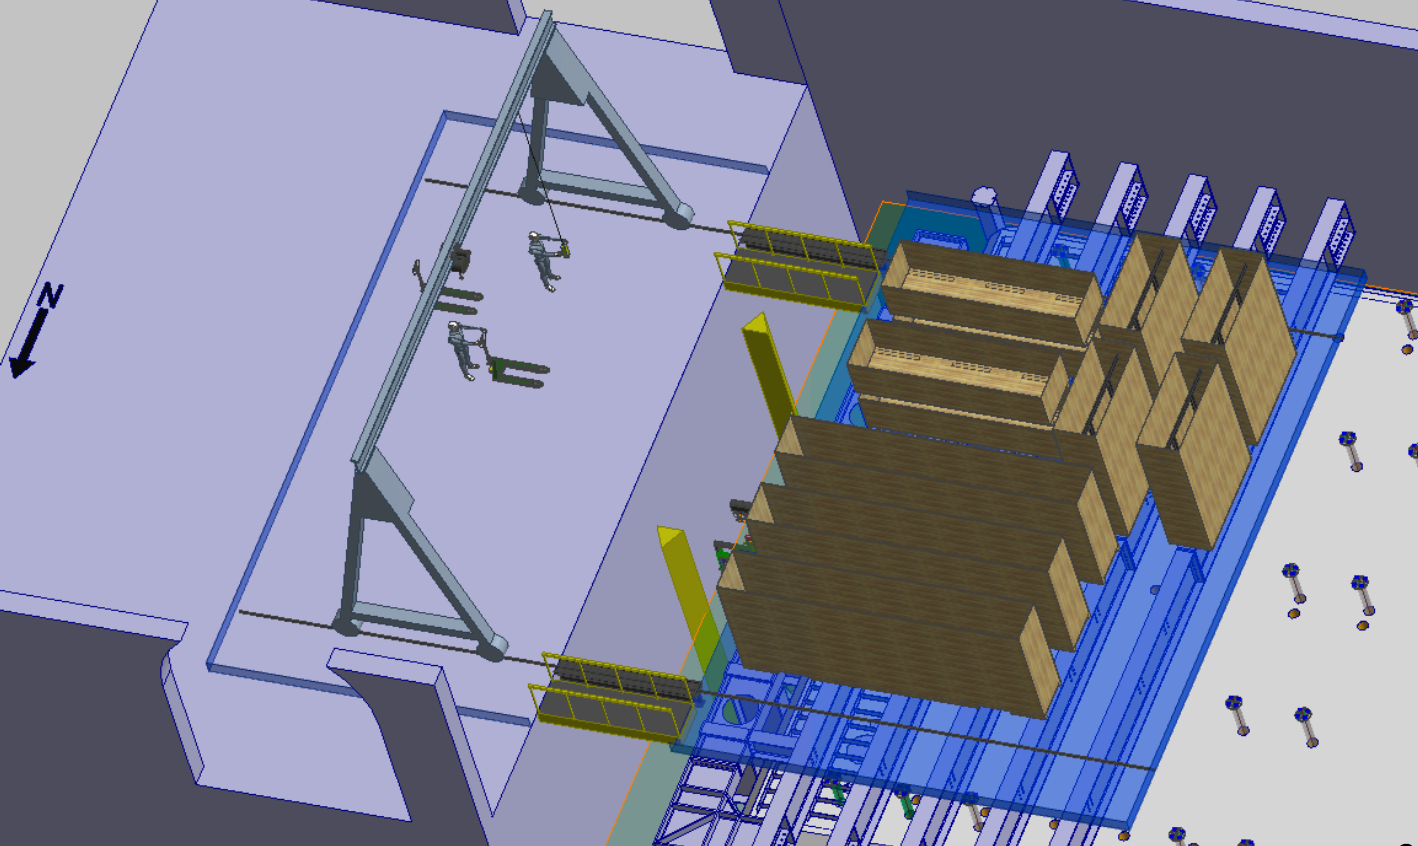
\includegraphics[height=0.26\textheight]{sp-apa-underground-storage.png}} 
\fbox{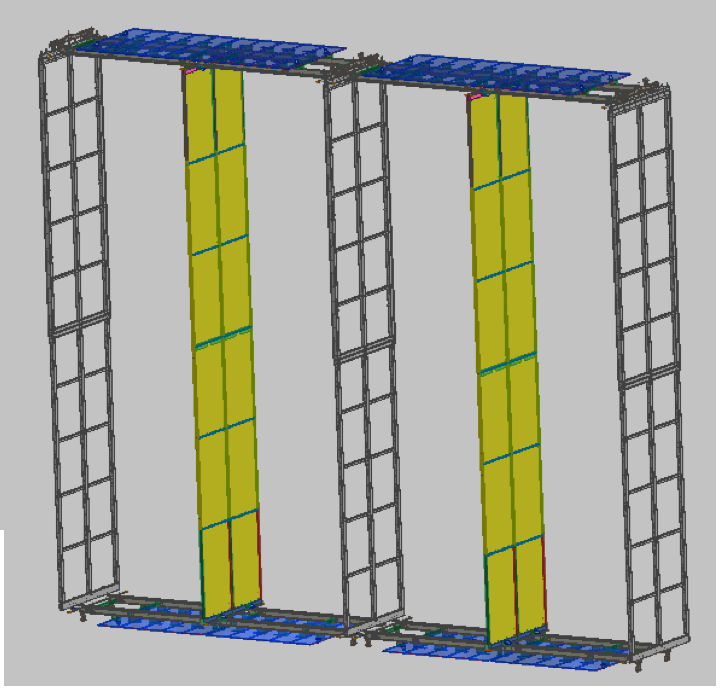
\includegraphics[height=0.26\textheight,trim=0mm 2mm 2mm 0mm,clip]{sp-apa-acaca-wall.png}}
\end{dunefigure}

%\paragraph{Tests underground in the \dword{tco} area}
Pairs of \dwords{apa} (top and bottom) are lowered in front of the \dword{tco} to be linked and cabled. Once the cabling is finished, a connection test is performed to ensure adequate cabling. The space near the \dword{tco} is very restricted (see Figure~\ref{fig:handling}), so no additional tests other than visual inspection are performed at that time, and the cabled and linked \dwords{apa} are positioned in their final location in the cryostat.

%\begin{dunefigure}[Schematics of the \dword{tco}  area]{fig:tco}{A schematic of the layout for the \dword{tco} area underground.}
%\begin{tabular}{cc}
%%\includegraphics[width=0.23\textwidth]{tco1.png} &
%%\includegraphics[width=0.3\textwidth]{tco2.png}
%\end{tabular}
%\end{dunefigure}

%\paragraph{Tests underground in the cryostat}
The current goal is to install a full APA-CPA-APA-CPA-APA wall every week (see Figure~\ref{fig:storage}, right). After each wall is installed, the night crew has time for final testing of the installed \dword{apa}. Currently, we have two testing models: one where the night crew tests \dword{apa} pairs as they are installed (every two days), and the other where the night crew tests the full wall at once. The decision will be made when accurate estimates of the time needed for testing become available.

%\begin{dunefigure}[Schematics of the wall in the cryostat]{fig:wall}{A schematic of the layout of a full \dword{apa}-\dword{cpa}-\dword{apa}-\dword{cpa}-\dword{apa} wall installed in the cryostat.}
%%\includegraphics[width=0.4\textwidth]{wall.png}
%\end{dunefigure}

The tests are %performed will be 
the same as described above at the \dword{itf}. Tension on a small set of wires is measured ($\sim$5\%, more if a quicker tension testing method is developed) to ensure that the installation operations did not alter the \dwords{apa}. With the complete integration now done, a full readout test can be performed. Short runs are taken with the \dword{daq} system to ensure that the readout is fully operational. The details of these tests must still be developed to provide efficient assessment of the integrated \dwords{apa}. If an \dword{apa} appears to have more than \num{1}\,\% of the channels not functioning, the \dword{apa} is sent back to the \dword{itf}.


%\subsubsection{Quality Assurance}
%We will rely on the \dword{pdsp} experience to assess most of the \dword{qa} protocols. The dedicated \dword{qa} plan during production should ensure that the \dwords{apa} meet the requirements and the installation steps should not modify them. The control of the quality of each wire along the installation steps will ensure fully functioning \dwords{apa}. The detailed \dword{qa} program is currently under development by the installation and integration group in the \dword{apa} consortium.

\end{comment}
